% Masters/Doctoral Thesis 
% LaTeX Template
% Version 2.5 (27/8/17)
%
% This template was downloaded from:
% http://www.LaTeXTemplates.com
%
% Version 2.x major modifications by:
% Vel (vel@latextemplates.com)
%
% This template is based on a template by:
% Steve Gunn (http://users.ecs.soton.ac.uk/srg/softwaretools/document/templates/)
% Sunil Patel (http://www.sunilpatel.co.uk/thesis-template/)
%
% Template license:
% CC BY-NC-SA 3.0 (http://creativecommons.org/licenses/by-nc-sa/3.0/)
%

%----------------------------------------------------------------------------------------
%	PACKAGES AND OTHER DOCUMENT CONFIGURATIONS
%----------------------------------------------------------------------------------------

\documentclass[
12pt, % The default document font size, options: 10pt, 11pt, 12pt
oneside, % Two side (alternating margins) for binding by default, uncomment to switch to one side
english, % ngerman for German
singlespacing, % Single line spacing, alternatives: onehalfspacing or doublespacing
%draft, % Uncomment to enable draft mode (no pictures, no links, overfull hboxes indicated)
%nolistspacing, % If the document is onehalfspacing or doublespacing, uncomment this to set spacing in lists to single
%liststotoc, % Uncomment to add the list of figures/tables/etc to the table of contents
%toctotoc, % Uncomment to add the main table of contents to the table of contents
parskip, % Uncomment to add space between paragraphs
%nohyperref, % Uncomment to not load the hyperref package
headsepline, % Uncomment to get a line under the header
chapterinoneline, % Uncomment to place the chapter title next to the number on one line
consistentlayout, % Uncomment to change the layout of the declaration, abstract and acknowledgements pages to match the default layout
]{MastersDoctoralThesis} % The class file specifying the document structure

\usepackage[croatian, english]{babel}
\usepackage[utf8]{inputenc} % Required for inputting international characters
\usepackage[T1]{fontenc} % Output font encoding for international characters

\usepackage{minted}
\usepackage{enumitem}
\usepackage{mathpazo} % Use the Palatino font by default

\usepackage{float}

\usepackage[backend=bibtex,style=numeric,natbib=true, sorting=none]{biblatex} % Use the bibtex backend with the authoryear citation style (which resembles APA)

\addbibresource{sources.bib} % The filename of the bibliography

\usepackage[autostyle=true]{csquotes} % Required to generate language-dependent quotes in the bibliography

\graphicspath{ {../gallery/} }

\selectlanguage{croatian}

%----------------------------------------------------------------------------------------
%	MARGIN SETTINGS
%----------------------------------------------------------------------------------------

\geometry{
	paper=a4paper, % Change to letterpaper for US letter
	inner=2.5cm, % Inner margin
	outer=3.8cm, % Outer margin
	bindingoffset=.5cm, % Binding offset
	top=1.5cm, % Top margin
	bottom=1.5cm, % Bottom margin
	%showframe, % Uncomment to show how the type block is set on the page
}

%----------------------------------------------------------------------------------------
%	THESIS INFORMATION
%----------------------------------------------------------------------------------------

\thesistitle{Globalna Iluminacija} % Your thesis title, this is used in the title and abstract, print it elsewhere with \ttitle
\supervisor{doc. dr. sc. Domagoj Ševerdija} % Your supervisor's name, this is used in the title page, print it elsewhere with \supname
\degree{Prvostupnik Matematike i Računarstva} % Your degree name, this is used in the title page and abstract, print it elsewhere with \degreename
\author{Antonio Janjić} % Your name, this is used in the title page and abstract, print it elsewhere with \authorname

\subject{} % Your subject area, this is not currently used anywhere in the template, print it elsewhere with \subjectname
\keywords{} % Keywords for your thesis, this is not currently used anywhere in the template, print it elsewhere with \keywordnames
\university{Sveučilište Josipa Jurja Strossmayera u Osijeku} % Your university's name and URL, this is used in the title page and abstract, print it elsewhere with \univname
\department{Odjel za Matematiku} % Your department's name and URL, this is used in the title page and abstract, print it elsewhere with \deptnameme
\faculty{Sveučilišni preddiplomski studij matematike i računarstva} % Your faculty's name and URL, this is used in the title page and abstract, print it elsewhere with \facname

\AtBeginDocument{
\hypersetup{pdftitle=\ttitle} % Set the PDF's title to your title
\hypersetup{pdfauthor=\authorname} % Set the PDF's author to your name
\hypersetup{pdfkeywords=\keywordnames} % Set the PDF's keywords to your keywords
}

\begin{document}

\frontmatter % Use roman page numbering style (i, ii, iii, iv...) for the pre-content pages

\pagestyle{plain} % Default to the plain heading style until the thesis style is called for the body content

%----------------------------------------------------------------------------------------
%	TITLE PAGE
%----------------------------------------------------------------------------------------

\begin{titlepage}
	\begin{center}

		\vspace*{.06\textheight}
		{\scshape\univname\par}\vspace{0.5cm} % University name
		\Large\deptname\\\facname\\[1cm]
		\textsc{\Large Završni praktični projekt - dokumentacija}\\[0.5cm] % Thesis type

		\HRule \\[0.4cm] % Horizontal line
		{\LARGE \bfseries \ttitle\par} % Thesis title
		\HRule \\[1.5cm] % Horizontal line

		\begin{minipage}[t]{0.4\textwidth}
			\begin{flushleft} \large
				\emph{Autor:}\\
				\authorname

			\end{flushleft}
		\end{minipage}
		\begin{minipage}[t]{0.4\textwidth}
			\begin{flushright} \large
				\emph{Mentor:} \\
				\supname

			\end{flushright}
		\end{minipage}\\[3cm]

		\vfill

		{\large Osijek, 2022.} % Date
		%\includegraphics{Logo} % University/department logo - uncomment to place it

	\end{center}
\end{titlepage}


%----------------------------------------------------------------------------------------
%	LIST OF CONTENTS/FIGURES/TABLES PAGES
%----------------------------------------------------------------------------------------

\tableofcontents % Prints the main table of contents

%----------------------------------------------------------------------------------------
%	THESIS CONTENT - CHAPTERS
%----------------------------------------------------------------------------------------

\mainmatter % Begin numeric (1,2,3...) page numbering

\pagestyle{thesis} % Return the page headers back to the "thesis" style

% Include the chapters of the thesis as separate files from the Chapters folder
% Uncomment the lines as you write the chapters

\chapter{Opis projekta}
Ovaj projekt je namijenjen kao implementacija raytracera sa globalnom iluminacijom, prvenstveno
kao što je opisano u knjizi \emph{"Advanced Global Illumination"} \cite{advGI}.

Projekt je u potpunosti implementiran u C++ jeziku.

{\let\clearpage\relax \chapter{Početak rada}}

\section{Ovisnosti}
Ovaj projekt ovisi o sljedećem softveru, kodovima i bibliotekama. Njihova instalacija prije
kompiliranja programa je nužna za rad.
\begin{itemize}
	\item \emph{premake5} za automatsku izradu konfiguracija.
	\item \emph{OpenMP} je potreban za paralelno izvršavanje u release buildu \\ programa.
	\item \href{https://github.com/g-truc/glm}{\emph{GLM}} se koristi za vektore, matrice i
	      operacije nad istim.
	\item Pomoćne klase i funkcije su uzete \href{https://github.com/Lame-een/LameUtil}{iz ove biblioteke}
	\item \href{https://github.com/nothings/stb}{stbimage}-jevi headeri za učitavanje i spremanje slika
\end{itemize}



\section{Preuzimanje}
Klonirajte repozitorij pomoću \\
\mintinline{shell}{git clone --recursive https://github.com/Lame-een/globalillum}

Ako je repozitorij bio kloniran ne rekurzivno ranije, koristite \\
\mintinline{shell}{git submodule update --init} \\
kako bi se klonirali potrebni podmoduli.



\section{Instaliranje}
\subsection{Windows}
Pokrenite \emph{premake5} pored \emph{premake5.lua} datoteke sa \emph{vs2022} argumentom
kako bi kreirali potrebne Visual Studio datoteke za development i za kompiliranje.

\subsection{Linux}
Pokrenite \emph{premake5} pored \emph{premake5.lua} datoteke sa \emph{gmake} argumentom
kako bi kreirali Makefile, koji se može koristiti za kompiliranje programa.

Zadana konfiguracija bi trebala producirati release build. Konfiguracija se može odabrati
postavljanjem make-ovog \emph{config} argumenta na \emph{config=release} ili
\emph{config=debug}.

\section{Korištenje programom}
Prema zadanim postavkama program će se izgraditi u \\
\mintinline{shell}{./bin/x64/%configuration%}
direktoriju.

Program se može pokrenuti u komandnoj liniji korištenjem sljedećih argumenata:
\begin{minted}{shell}
	GIrt.exe [OPTIONS] output_image_name
\end{minted}

Postavke programa se mogu zadati dodavanjem \emph{OPTIONS} zastava.

Popis svih zastava:
\begin{itemize}
	\item Postake raytracera: \\
	      \begin{tabular}{ l l }
		      \mintinline{shell}{-help}                     & Prikaže zaslon s pomoći.                                                 \\
		      \mintinline{shell}{-s, -samples}              & Postavi broj uzoraka po pikselu. (\emph{1024})                           \\
		      \mintinline{shell}{-depth}                    & Postavi maksimalnu dubinu rekurzije. (\emph{25})                         \\
		      \mintinline{shell}{-w, -width}                & Postavi širinu slike. (\emph{640})                                       \\
		      \mintinline{shell}{-h, -height}               & Postavi visinu slike. (\emph{640})                                       \\
		      \mintinline{shell}{-fov}                      & Postavi Field Of View kamere (u stupnjevima). (\emph{60})                \\
		      \mintinline{shell}{-bg, -background}          & Postavi pozadinu scene u hex RGB. (\emph{"\#3a3a3a"})                    \\
		      \mintinline{shell}{-bgimg, -background-image} & Postavi pozadinu scene na \textbf{day} ili \textbf{night}. (\emph{none}) \\
		      \mintinline{shell}{-gamma}                    & Postavi korekciju game za sliku. (\emph{2.2})
	      \end{tabular}
	\item Postavke za primjere: \\
	      \begin{tabular}{ l l }
		      \mintinline{shell}{-demo}      & Odaberi jedan od postojećih primjera scene. \\
		      \mintinline{shell}{-demo-list} & Izlistaj sve postojeće primjere scena.
	      \end{tabular}
\end{itemize}

(Napomena: Sve zastave i postavke su osjetljive na veliko i malo slovo.)

Izlazna slika će se nalaziti u \mintinline{shell}{./out} direktoriju. Direktoriji će biti
stvoren pokraj same executeable datoteke.

\vspace{2cm}

Primjer korištenja:

\mintinline{shell}{GIrt.exe -help} \quad -- Prikaže sve moguće CLI argumente.

\mintinline{shell}{GIrt.exe -w 250 -h 250 -demo 0 demo_0_render} \quad -- Postavi širinu i visinu
slike na 250 piksela, započne renderanje primjera broj 0 i spremi sliku kao \emph{"demo\_0\_render.png"}

\vspace{2cm}

{\let\clearpage\relax \chapter{Implementacija}}

\section{Opis rada}
Program je raytracer koji koristi Monte Carlo integraciju za aproksimiranje globalne iluminacije.
Kao u standardnom raytraceru zrake svijetla se šalju iz točke koja simulira senzor kamere
ili retinu oka. Zrake se šalju kroz svaki piksel i uz to za svaki piksel se pošalje
zadani broj uzoraka zraka koje su sve blago perturbirane unutar piksela.
%TODO add image describing the process

Svaka zraka se provjeri na presjek sa objektom ili pozadinom scene. Pri presjeku sa objektom
informacije o hitcu su spremljene u \emph{HitInfo} klasi i materijal objekta će vratiti podatke
o raspršenju zraka pomoću \emph{ScatterInfo} klase.
%TODO maybe another image here?

Sa podatcima u \emph{ScatterInfo} klasi možemo nastaviti rekurzivno slati zrake iz točke sjecišta
oviseći o tome kakva je interakcija između zrake i materijala.

Odašiljane zrake nose informacije o boji/luminaciji natrag pomoću rekurzije, sve zrake po pikselu
u prosjeku daju boju tog piksela slike.

Dodatno je implementirana i aproksimacija Fresnellovog efekta za prozirne materijale.

\vspace*{2cm}

%%todo check grammar after this
U nastavku ću napraviti kratak opis struktura, klasa i funkcija koje su implementirane. Za
potpune informacije pogledajte sam kod na \href{https://github.com/Lame-een/globalillum}{repozitoriju}.

\section{Namespaces}

\subsection*{Colors}
\emph{Colors} namespace enkapsulira definirane konstante izraze za različite boje.

Omogućuje jednostavno korištenje osnovnih boja bez da se svaki puta moraju manualno unositi hex
kodovi boja.

Primjer gdje se koristi namespace:
\begin{minted}[linenos]{cpp}
    //primjer iz ./src/demos/cornellBoxWindow.h
    ...
    Diffuse matUpDown(StringToRGB("#808080"));
    Diffuse matLeft(Colors::crimson);
    ...
\end{minted}
Vidimo kako za razliku od linije 3, u liniji 4 možemo iskoristiti samo naziv boje unutar namespacea
\emph{Colors}.

\subsection*{Settings}
Ovaj namespace enkapsulira globalne varijable koje služe kao reprezentacija postavki i funkcije
za rad nad postavkama.

Ova klasa se u budućnosti može pretvoriti u Singleton object, no za vrijeme izrade projekta bilo
je jednostavnije koristiti namespace.

\section{Klase}

\subsection*{Object}
\emph{Object} klasa je bazna klasa za sve objekte koji se mogu nalaziti u sceni.

Deklarirana je na sljedeći način:
\begin{minted}[linenos]{cpp}
class Object
{
public:
	Object(bool cull = true, bool samplingTarget = false);
	Object(const Material* mat, bool cull = true, 
	       bool samplingTarget = false);

	virtual bool Hit(const Ray& ray, double tMin, 
	                 double tMax, HitInfo& hitInfo) const;

	virtual bool BoundingBox(AABB& outputBox) const;

	virtual Vec3 Random(Vec3 point) const;
	virtual double PdfValue(const Vec3& origin, const Vec3& dir) const;

	bool IsSamplingTarget() const;

	const Material* GetMaterial() const;
protected:
	const Material* m_Mat = nullptr;

	bool m_Cull;
	bool m_SamplingTarget;
};
\end{minted}

Konstruktor vidljiv u liniji 5 prima pokazivač na materijal objekta, te dvije boolean vrijednosti: 
\texttt{cull} zadaje hoće li se vršiti \emph{backface culling} nad objektu, 
\texttt{samplingTarget} zadaje hoće li se objekt dodatno uzimati u obzir pri uzorkovanju zraka.

\begin{minipage}{\textwidth}
\begin{minted}{cpp}
virtual bool Hit(const Ray& ray, double tMin, 
                 double tMax, HitInfo& hitInfo) const;
\end{minted}

je funkcija koju je nužno implementirati u deriviranim
objektima. Poziva se pri ispitivanju siječe li zraka \texttt{ray} sam objekt i vraća \emph{true}
ako siječe.
\end{minipage}
\\

\begin{minted}{cpp}
virtual bool BoundingBox(AABB& outputBox) const
\end{minted}
se koristi za stvaranje kvadra poravnatog s osima koji omeđuje sam objekt.
\\

\begin{minted}{cpp}
virtual Vec3 Random(Vec3 point) const
\end{minted}
se koristi za generiranje nasumičnog vektora koji pokazuje prema objektu.
\\

\begin{minted}{cpp}
virtual double PdfValue(const Vec3& origin, const Vec3& dir) const
\end{minted}
se koristi za generiranje funkcije gustoće vjerojatnosti za objekt pri uzorkovanju.
\\

Klase \textbf{Sphere}, \textbf{Triangle}, \textbf{TriangleMesh} su derivirane klase klase Object.
Dok klasa \textbf{Quad} je derivirana klasa klase TriangleMesh i implementira trodimenzionalni
četverokut. Za više detalja o pojedinim klasama pogledajte repozitorij.

\vspace*{2cm}

\subsection*{Material}

\begin{minipage}{\textwidth}

	\emph{Material} je bazna klasa pomoću koje se mogu stvoriti materijali objekata.

\begin{minted}[linenos]{cpp}
class Material
{
public:
	Material(bool isEmissive = false, 
             bool isTransmissive = false);
	virtual RGB Emit(const Ray& incidentRay,
                     const HitInfo& hitInfo) const;

	virtual bool Scatter(const Ray& incidentRay, 
	                     const HitInfo& hitInfo,
                         ScatterInfo& scatterInfo) const;
	virtual double ScatterPDF(const Ray& incidentRay, 
                              const HitInfo& hitInfo,
                              const Ray& scatterRay) const;

	static const Material* Default();

	bool IsEmissive() const;
	bool IsTransmissive() const;

private:
	bool m_Emissive;
	bool m_Transmissive;

	static Material s_DefaultMat;
};
\end{minted}
\end{minipage}

Konstruktor ove klase prima dva argumenta. \texttt{isEmissive} deklarira može li ovaj materijal
emitirati svijetlost, dok \texttt{isTransmissive} deklarira hoće li ovaj objekt propuštati
zrake.
\\

\begin{minted}{cpp}
virtual RGB Emit(const Ray& incidentRay, 
                 const HitInfo& hitInfo) const
\end{minted}
je funkcija koja se implementira u materijalima koji emitiraju svijetlost. Za sve ostale
materijale može ostati ne implementirana i preuzeta iz bazne klase.

\begin{minted}{cpp}
virtual bool Scatter(const Ray& incidentRay, 
                     const HitInfo& hitInfo, 
                     ScatterInfo& scatterInfo) const
\end{minted}
jer virtualna funkcija koja se implementira u konkretnim materijalima i zadaje kako će se
zraka \texttt{incidentRay} raspršiti pri hitcu. Rezultantna zraka se sprema u 
\texttt{scatterInfo}.


\begin{minted}{cpp}
virtual double ScatterPDF(const Ray& incidentRay,
                          const HitInfo& hitInfo, 
                          const Ray& scatterRay) const
\end{minted}
vraća vrijednost funkcije gustoće vjerojatnosti za pojedini materijal.

\vspace*{1cm}
Trenutno su implementirani sljedeći materijali: \textbf{Diffuse}, \textbf{Specular},
\textbf{Transmissive} i \textbf{Light}. Svaka pojedina od tih klasa derivira je od Material 
klase i implementira virtualne funkcije na prikladan način.

\vspace*{2cm}

\subsection*{AABB}

Osno poravnati granični okvir (eng. Axis-Aligned Bounding box) je klasa koja opisuje kvadar
koji omeđuje neki objekt. Koristi se za ubrzanje određivanja pogotka zrake sa objektom.

\begin{minted}[linenos]{cpp}
class AABB
{
public:
	AABB();
	AABB(const Vec3& min, const Vec3& max);

	const Vec3& Min() const;
	const Vec3& Max() const;

	const void Set(const Vec3& min, const Vec3& max);

	bool Hit(const Ray& r, double tMin, double tMax) const;
	void Surround(const AABB& box);

private:
	Vec3 m_Min = Vec3(0);
	Vec3 m_Max = Vec3(0);
};
\end{minted}

Konstruktor ove klase prima dvije točke u 3D prostoru koje predstavljaju "najmanju" i "najveću"
točku kvadra.

\begin{minted}{cpp}
bool Hit(const Ray& r, double tMin, double tMax) const
\end{minted}
vraća prolazi li zraka \texttt{r} kroz okvir. Funkcija je implementirana po uzoru na Andrew
Kensler-ovu implementaciju \cite{kensler}.

\begin{minipage}{\textwidth}
\begin{minted}{cpp}
void Surround(const AABB& box)
\end{minted}
je funkcija koja uspoređuje okvir koji poziva funkciju sa \texttt{box} okvirom. Funkcija određuje
okvir koji opisuje ta dva te postavlja trenutni na taj veći.
\end{minipage}

\subsection*{BVHNode}
Klasa \emph{BVHNode} je derivirana klasa klase Object. Njezina uloga je kao gradivni dio za
hijerarhiju ograničavajućeg volumena (eng. Bounding Volume Hierarchy - BVH).

BVH je reprezentacija objekata u nekoj dimenziji pomoću stabla. Ovdje je korištena za brzi
pronalazak pogotka zrake sa objektima u sceni.

BVH je implementiran na način da se konstruira binarno stablo pri čemu su listovi objekti unutar
scene. Pri grananju se nasumično odabire dimenzija po kojoj će se uspoređivat dva AABB-a i tako
se određuje hoće li skup objekata biti u lijevom ili desnom djetetu stabla.

Za detalje vidite potpunu implementaciju u \texttt{"./src/objects/bvh.cpp"}


\subsection*{HitInfo i ScatterInfo}
Ove dvije strukture se koriste za prijenos podataka o presjeku zrake i objekta, te o raspršenju
zrake pri hitcu od objekt.

\begin{minted}[linenos]{cpp}
struct HitInfo
{
public:
	Vec3 point;
	Vec3 normal;
	const Object* object = nullptr;
	double t;
};
\end{minted}
\begin{description}[labelindent=1cm]
	\item[point] je točka u kojoj je došlo je presjeka.
	\item[normal] je normala na točku presjeka.
	\item[object] je pokazivač na objekt koji je pogođen.
	\item[t] je dužina zrake koja je pogodila objekt.
\end{description}

\vspace*{1cm}

\begin{minted}[linenos]{cpp}
class ScatterInfo
{
public:
	~ScatterInfo();

	Ray bounceRay;
	bool isSpecular;
	RGB color;

	const PDF* Pdf() const;
	void SetPdf(PDF* ptr);
private:
	const PDF* m_pdf = nullptr;
};
\end{minted}
\begin{description}[labelindent=1cm]
	\item[bounceRay] je zraka koja se stvorila pri raspršenju.
	\item[isSpecular] specificira je li ova zraka prozirna ili spekularna.
	\item[color] je boja zrake.
	\item[m\_pdf] sadrži funkciju gustoće vjerojatnosti zrake. 
\end{description}


\vspace*{2cm}

\subsection*{Camera i Viewport}
Ove dvije klase implementiraju kameru i prozor za prikaz slike \\ 
(eng. viewport) scene.

\emph{Camera} je jednostavna klasa koja se konstruira pomoću sljedećeg konstruktora:
\begin{minted}{cpp}
Camera(const Vec3& pos, const Vec3& dir, const Vec3& up)
\end{minted}
\texttt{pos} je pozicija kamere, \texttt{dir} je smjer u kojem kamera gleda, \texttt{up} je
vektor smjera koji izlazi iz gornje strane kamere. 

\emph{Viewport} je klasa koja služi za projekciju zraka na "površinu unutar kamere". Zapravo je
struktura koja će spremati podatke o slici koja se želi kreirati (širina i visina te FOV) i uz
kameru pomaže za operacije koje su potrebne za određivanje zraka koje se šalju u scenu.

\subsection*{Image}
\emph{Image} klasa sadrži sve nužne opracije nad ulaznim i izlaznim slikama. Implementirana
je na sljedeći način:
\begin{minted}[linenos]{cpp}
class Image{
public:
	Image(size_t width, size_t height);
	Image(const std::string& path);
	~Image();	

	void SetPixel(int x, int y, const RGB& color);
	RGB GetPixel(int x, int y);
	RGB GetPixel(double u, double v);

	const Vec2i& Dimensions();
	bool IsLoaded() const;
	bool HasData() const;

	void WriteFile(const std::string& path);
private:
	Vec2i m_Dimensions;
	double m_Gamma;
	bool m_Loaded;

	unsigned char* m_Bitmap = nullptr;
};
\end{minted}

Vidimo kako postoje dva konstruktora. Prvi
\begin{minted}{cpp}
Image(size_t width, size_t height)
\end{minted}
kreira praznu sliku širine \texttt{width} i visine \texttt{height}. Pikseli se mogu lagano
bojati koristeći
\begin{minted}{cpp}
void SetPixel(int x, int y, const RGB& color)
\end{minted}
funkciju. Tako kreirana slika se zatim može spremiti kao datoteka na putanji \texttt{path} 
koristeći:
\begin{minted}{cpp}
void WriteFile(const std::string& path)
\end{minted}

Drugi konstruktor:
\begin{minted}{cpp}
Image(const std::string& path)
\end{minted} 
učitava sliku sa putanje \texttt{path}.

\subsection*{Cubemap}
\emph{Cubemap} klasa enkapsulira 6 slika koje čine "environment map" scene. Koristi se vrlo lako.
Konstruktor klase prihvaća putanju do direktorija u kojoj se nalazi 6 slika koje čine cubemap.
Sa tako konstruiranom klasom uz pomoć funkcije
\begin{minted}{cpp}
RGB Sample(const Vec3& dir) const
\end{minted}
koja prima vektor smjera može se uzorkovat boja koja se nalazi u "okolišu" u tom smjeru.

\subsection*{PDF}
\emph{PDF} je bazna klasa za implementiranje funkcije gustoće vjerojatnosti.
\begin{minted}[linenos]{cpp}
class PDF
{
public:
	virtual double Value(const Vec3& dir) const = 0;
	virtual Vec3 Generate() const = 0;
};
\end{minted}
Deklarira dvije čiste virtualne funkcije koje se trebaju implementirati u deriviranim klasama.
Trenutne implementirane bazne klase su: \textbf{CosinePDF}, \textbf{SpecularPDF}, \textbf{ObjectsPDF}
\textbf{MixturePDF}.

\subsection*{ONB}
\emph{ONB} je pomoćna klasa za izgradnju ortonormirane baze. Konstruira se pomoću normale koja
postaje vektor "gore" unutar baze.

Klasa je izuzetno korisna za generiranje vektora unutar \emph{PDF} klasa.

Implementacija je napravljena po uzoru na članak \emph{"Building an Orthonormal Basis, Revisited"}\cite{ONBrevisited}.

\subsection*{Scene}
\emph{Scene} je jedna od najbitnijih klasa u cijelom programu. Sadrži sve objekte koji su stvoreni
i obavlja rad vezan za provjeru sjecišta zrake i objekta.

Napomena: bitno je pozvati funkciju
\begin{minted}{cpp}
void ConstructBvh()
\end{minted}
prije poziva \texttt{Raytracer} funkcije, inače neće se izvršiti izgradnja BVH stabla.

Unatoč tome što sama klasa nije previše komplicirana, ipak je velika te ostavljam detalje
implementacije u header i source fileu na repozitoriju.

\section{Funkcije}

\subsection*{Raytracer}
Funkcije
\mintinline{cpp}{void RayTracer(const Viewport& vp, const Scene& scene)} i \\
\mintinline{cpp}{RGB TraceRay(const Scene& scene, const Ray& ray, int depth = 0)} su dvije osnovne
funkcije potrebne za funkcionalnost.

\texttt{RayTracer} funkcija obavlja prolazak kroz piksele slike te generiranje zraka koji izlaze
iz kamere.

\texttt{TraceRay} je rekurzivna funkcija koja obavlja praćenje zrake kroz scenu i sve interakcije
koje zraka može učiniti.

\subsection*{Matematičke funkcije}
Implementirano je nekoliko pomoćnih matematičkih funkcija.

\begin{minted}{cpp}
bool solveQuadratic(const double& a, const double& b, const double& c, 
                    double& x0, double& x1)
\end{minted}
je funkcija koja preko \texttt{x0} i \texttt{x1} vraća rješenja kvadratne jednadžbe.

Funkcije \texttt{SchlicksApprox} računaju aproksimaciju Fresnellovog koeficijenta refleksije.

Implementiran je i skup funkcija za nasumično generiranje točaka/smjerova:
\begin{description}
	\item[\mintinline{cpp}{RandomCosineDir()}] -- generira smjer unutar hemisfere prema 
		kosinusovoj distribuciji.
	\item[\mintinline{cpp}{RandomSpecularDir(double shininess)}] -- generira nasumični smjer prema
		spekularnoj distribuciji (implementacija po izvještaju Erica P. Lafortune \cite{lafortune}).
	\item[\mintinline{cpp}{PointInUnitSphere()}] -- generira nasumičnu točku unutar jedinične sfere.
	\item[\mintinline{cpp}{PointInUnitCircle()}]  -- generira nasumičnu točku unutar jedinične kružnice.
	\item[\mintinline{cpp}{PointInCone(double radius, double sqrDist)}] -- generira nasumičnu točku
		unutar stošca kvadratne visine \texttt{sqrDist} i radijusa baze \texttt{radius}.
\end{description}

{\let\clearpage\relax \chapter{Za developere}}

\section{Stil koda}
Ovaj projekt koristi varijantu Microsoft-ovog stila. Za generalniji pogled u stil molim pogledati
već postojeći codebase.

Napomena: implementacije klasa unutar header fileova bi se trebale izbjegavati.

\section{Konvencije nazivlja}
Klase, funkcije, metode, enums, namespaces su uvijek u \emph{PascalCase}.
Dozvoljava se da pomoćne funkcije budu u \emph{camelCase} u slučaju da su "privatne", tj.
korištene od drugih funkcija i ne očekuje se da će se pozivati u više funkcija.

\begin{itemize}
	\item Lokalne varijable i parametri funkcije su \textbf{uvijek} \emph{camelCase}.
	\item Privatne varijable klasa se prefiksiraju sa \emph{"m\_"} i započinju sa velikim slovom.
	\item Statične varijable se prefiksiraju sa \emph{"s\_"} i započinju sa velikim slovom.
\end{itemize}

\vspace{2cm}

Primjer stila:
\begin{minted}{cpp}
namespace ExampleNamespace{
    static int s_StaticInt = 0;

    static void StaticFunction();

    class ExampleClass
    {
        public:
        void MemberFunction(int var)
        {
            m_MemberVar = var;

            std::vector<int> localVector;
            localVector.push_back(var);
        }
    private:
        int m_MemberVariable = 0;
    };
}
\end{minted}

\section{Organizacija koda}
Sve datoteke moraju biti \emph{camelCase}. Moraju se nalaziti u \emph{./GIrt/src} direktoriju
i njihovi pripadajući header fileovi moraju biti pokraj njih u istom direktoriju.

Pomoćne klase, funkcije i drugi objekti trebali bi se nalaziti u \\
\emph{./GIrt/src/util} direktoriju.

Vendor fileovi i druge datoteke o kojima projekt ovisi \textbf{moraju} biti u \\
\emph{./GIrt/vendor}
direktoriju.




\chapter{Galerija}

Sve slike u ovom poglavlju su renderane sa 2000 uzoraka po pikselu, te su 900px široke i visoke.

\begin{figure}[h]
	\caption{Primjer difuznih interakcija.}
	\centering
	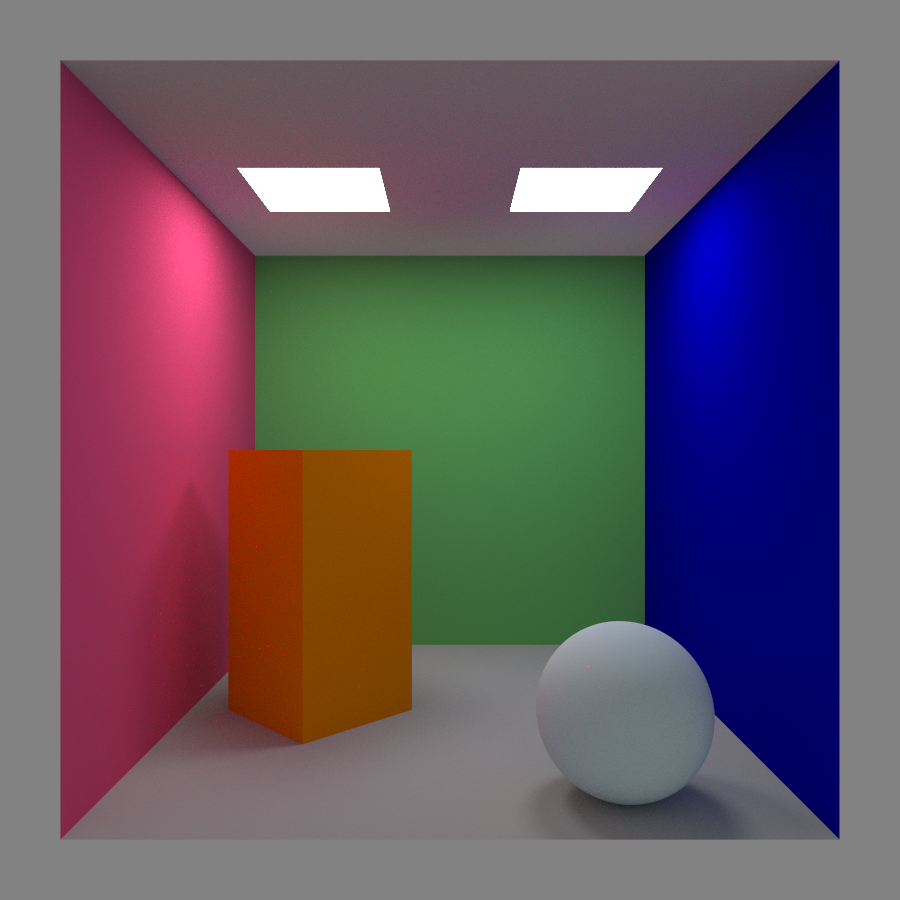
\includegraphics[width=\textwidth]{demo0.png}
\end{figure}

\begin{figure}[h]
	\caption{Primjer prozirnih interakcija.}
	\centering
	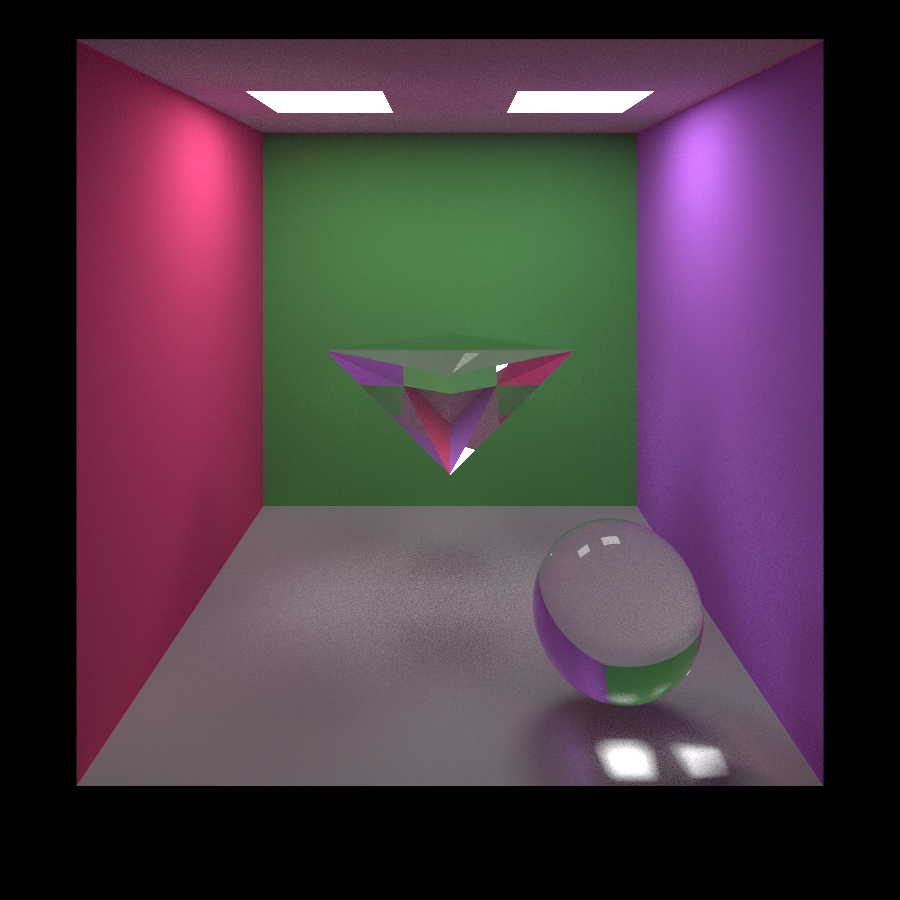
\includegraphics[width=\textwidth]{demo1.png}
\end{figure}

\begin{figure}[h]
	\caption{Primjer spekularnih interakcija sa hrapavostima materijala 0.01 i 0.5.}
	\centering
	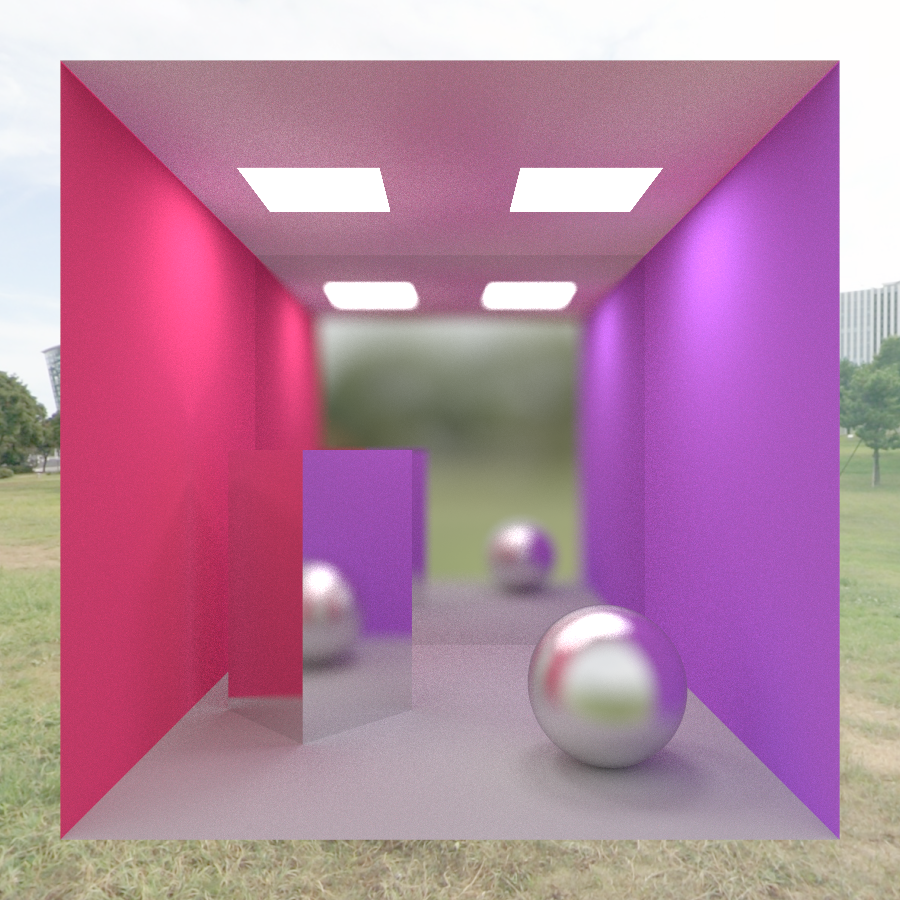
\includegraphics[width=\textwidth]{demo2.png}
\end{figure}

\begin{figure}[h]
	\caption{Primjer globalne iluminacije pomoću vanjskog svijetla iz cubemap-a.}
	\centering
	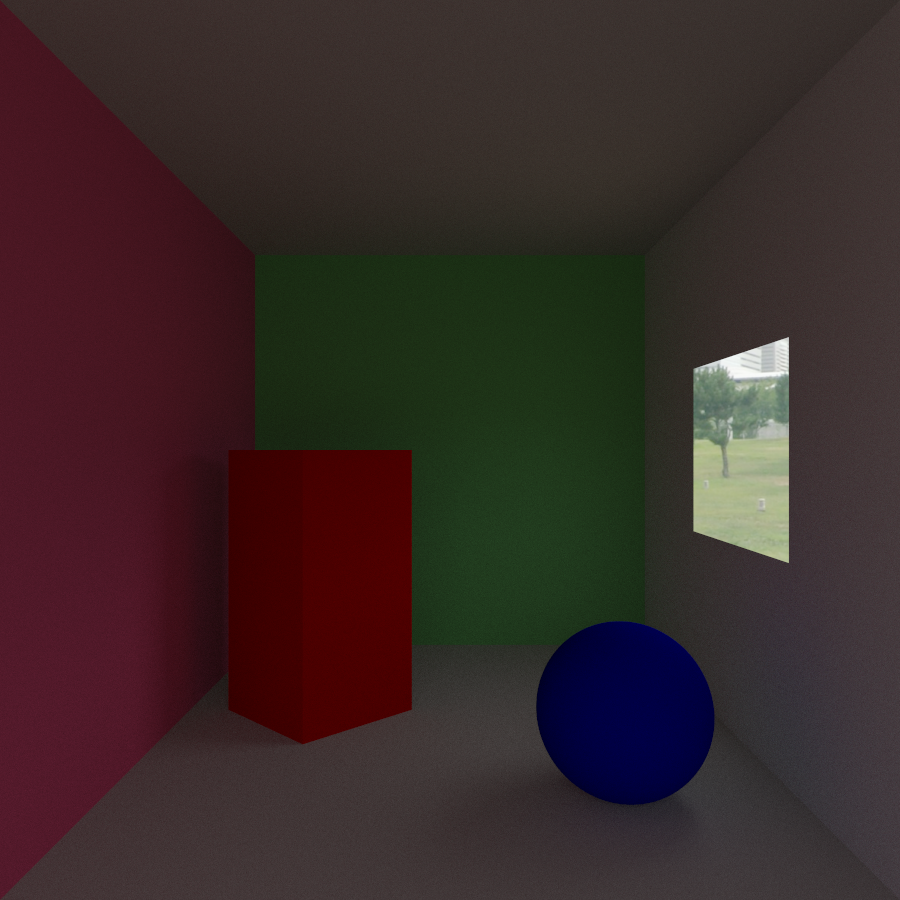
\includegraphics[width=\textwidth]{demo3.png}
\end{figure}

\begin{figure}[h]
	\caption{Primjer 3 metalne kugle - spekularne refleksije cubemapa.}
	\centering
	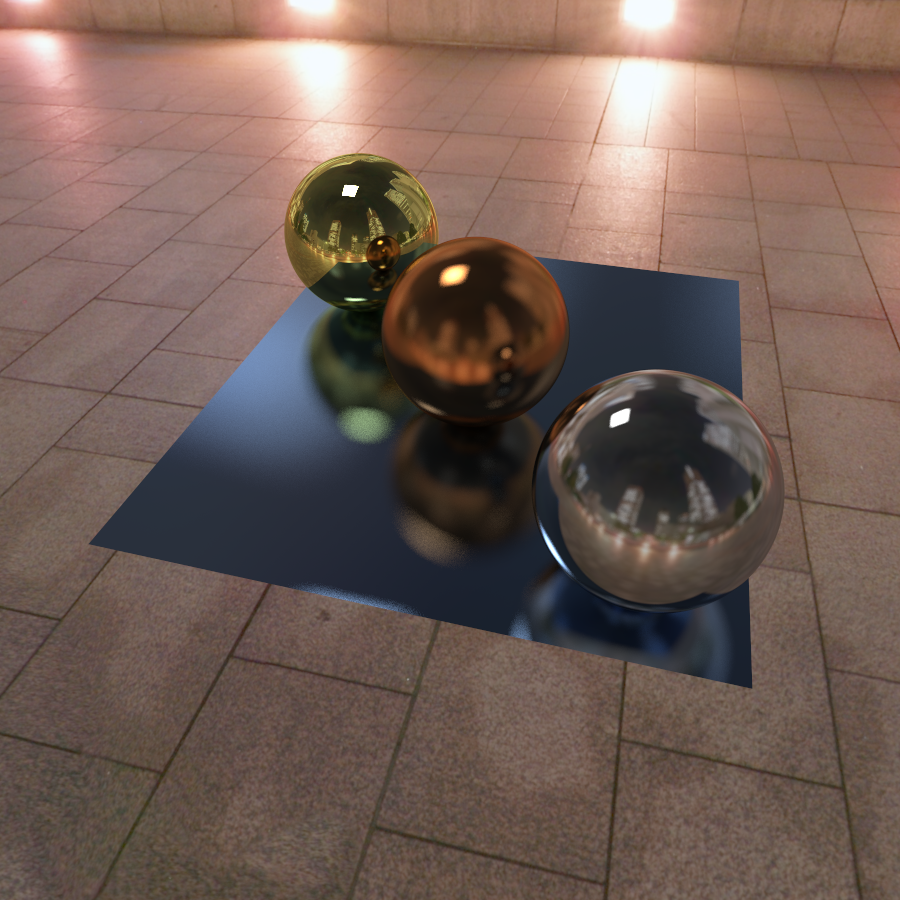
\includegraphics[width=\textwidth]{demo4.png}
\end{figure}

\chapter{Budući planovi}

Ovo je vrlo rudimentarna implementacija raytracera sa globalnom iluminacijom. Projekt služi
više kao proučavanje teme i motivacija za budući development.

No, postoji nekoliko funkcionalnosti koje bi se idealno implementirale kako bi projekt postao
koristan umjetnicima:
\begin{description}
	\item[Učitavanje modela iz datoteka] Trenutna implementacija zahtjeva ručno definiranje
		mreža trokuta i drugih objekata. Idealno bi bila mogućnost učitavanja .obj datoteka 
		(i pripadnih materijala) pozivom funkcije.
	\item[Učitavanje scene iz datoteke] Trenutna implementacija nema način uživog učitavanja
		scene iz datoteke, već zahtjeva ručno mijenjanje \emph{sandbox.h} datoteke i ponovno kompiliranje.
	\item[Novi materijali] Trenutno su implementirani difuzni, spekularni, prozirni i svijetleći
		materijal. Idealno bi bilo dodati dodatne materijale kao što su glossy i semi-prozirni
		materijal.
	\item[Podrška za teksture] Teksture, HDRIs, normal maps, displacement maps, UV mapiranje, itd.
		nisu trenutno podržani.
	\item[Interaktivni prozor za scene] Idealno bi bilo dodati mogućnost micanja objekata
		za vrijeme korištenja programa te renderanje tako kreirane scene.
	\item[Optimizacije] Program trenutno se potpuno izvršava na CPU, idealno bi bilo iskoristiti
		tehnologije kao što su CUDA ili OpenCL da se postignu kraća vremena renderanja.
	\item[Potpuni API reference] Trenutna dokumentacija nema potpunu API referencu. Sam izvorni 
		kod ima određene dijelove dokumentirane pomoću Doxygen-a, no ne cijeli codebase.
	\item[Vlastita implementacija paralelizacije] Trenutna implementacija koristi \\ 
		OpenMP za paralelizaciju izvršavanja. Idealno bi bilo implementirati vlastito 
		paralelno izvršavanje radi veće kontrole.
	\item[Mnoge druge...]
\end{description}






\chapter{Licence}

\begin{itemize}
	\item GLM koristi "The Happy Bunny License", za detalje vidite \href{https://github.com/g-truc/glm/blob/master/copying.txt}{ovdje}
	\item stb\_image koristi "MIT license", za detalje vidite \href{https://github.com/nothings/stb/blob/master/LICENSE}{ovdje}
	\item Projekt uključuje 2 cubemap-a Emila "Humus" Perssona, koje su licencirane pod CC BY 3.0 licencom
	      za dodatne informacije pogledajte njegovu \href{http://www.humus.name/index.php?page=Textures}{webstranicu}.
\end{itemize}


%----------------------------------------------------------------------------------------
%	BIBLIOGRAPHY
%----------------------------------------------------------------------------------------
\renewcommand{\bibname}{Literatura}
\nocite{basicsCG}
\nocite{weekend}
\printbibliography[heading=bibintoc]

%----------------------------------------------------------------------------------------

\end{document}
